\documentclass[11pt,dvipdfmx]{jarticle}
\usepackage{eee}
\usepackage{subfig}
\usepackage{url}

\begin{document}

\begin{jikkenTitle}
  \gakunen{3} % 学年を記述。この行で全体の枠を表示
  \numTitle{2}{ダイオードの特性} % 実験番号、タイトルを記述
  \subTitle{第1週 ダイオード ツェナーダイオード} % サブタイトルがあれば記述
  \jikkenbi{令和4年5月12日(木)} % 実験日を記述
  %\jikkenbiII{平成28年7月6日(木)} % 実験日を記述(二日目がある場合。ない場合はこの行をコメントアウト)
  \kyoudou{3302 新川\,史人, 3310 岡村\,放} % 共同実験者名を記述
  \kyoudouII{3318 鈴木\,春香 3327 猶崎稜真} % その他の共同実験者名を記述
  \yoteibi{5/19}% 予定日を記述
  \yoteibiII{}% 予定日2を記述
  \yoteibiIII{}% 予定日3を記述
  \hanNumberName{2班}{3314}{城戸 貴博} % 班番号・学生番号・氏名を記述。この行でタイトルページの描画を終了
\end{jikkenTitle}% 表紙

\section{目的}
今回の実験では以下の3点を目的とする。
\begin{itemize}
	\item ダイオードの原理を知り,実験により整流作用を理解することでダイオードを使用できるようにする。
	\item ツェナーダイオードの特性を学び,ツェナーダイオードを使用できるようにする。
	\item 太陽電池の特性を知り,使用できるようにする。
\end{itemize}

\section{原理}
\section{原理}
\subsection{LabVIEW}
NATIONAL INSTRUMENTS(NI)が提供しているLabVIEWは,各種計測器やmyRIOなどを用いて自動計測や制御を実装するためのグラフィカルユーザーインターフェイスのプログラミング言語である.
主な特徴は,ビルトインされた仮想計測器(Virtual Instruments,以下VI)で,オシロスコープやマルチメーターなどの計測器と似た外観や機能をコンピューター上へ作成するというものである.
VIは,フロントパネル,ブロックダイアグラム,アイコン-コネクタという3つ主要素から構成される.
プログラミングは,ブロックダイアグラム上にアイコンを配置し,各アイコン間のコネクタをつなぐ形で行う.

\subsection{myRIO}
myRIOは,デュアルコアのARM Cortex-A9 リアルプロセッサとカスタマイズ可能なXilinx FPGA・アナログプロセッサの駆動するプログラミング言語には,LabVIEWを用いる.
LabVIEWとmyRIOを用いることにより,制御,ロボット,メカトロニクス,組込などを容易に実現することができる.

\subsection{myRIO ブレッドボードアクセサリ}
myRIOの拡張ポートに接続可能なブレッドボードアクセサリ.
myRIOの5V,3.3V,GND端子及びAnalog I/O,Digital I/Oの端子が,ブレッドボード上に結線した回路とヘッダにマッピングされている.
そのため,ブレッドボード上に結線した回路とヘッダとをジャンパ線で結線することにより,回路への入出力制御および計測がmyRIOを用いて容易に実行することができる.

\subsection{可変抵抗器(ポテンショメータ)\cite{23r234r2}}
可変抵抗器(Potentiometer)は抵抗値を変更できる抵抗器の一種で,機械的な位置の変化をアナログ電気信号に変換することができる.
つまみを回すことにより,\wfig{ALPS}のように抵抗体の長さが変化することにより,抵抗値の変更が可能となっている.

\begin{figure}[h]
\centering
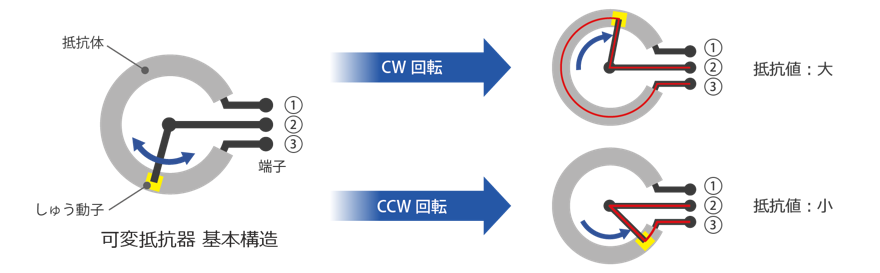
\includegraphics[scale=0.5]{/Users/ohyamasan/Downloads/TMCIT-Report/EE_Measurement/fig/pote_lp_01_02.png}
\caption{可変抵抗器の原理}
\label{fig:ALPS}
\end{figure}

\subsection{CdSセンサ\cite{dsfase}\cite{8347ty34i}\cite{B056}\cite{R300000001-I023994699-00}}
\label{CDSG}
光可変抵抗器ともいう.光電効果(photoelectric effect)である光導電性を利用し,光の強さで抵抗値が変化するCdS(硫化カドミウム)の性質を利用した電子部品.
光導電性は半導体の表面に光を当てるとキャリアが増加し,抵抗率が下がる現象である.
そのため,セルに当たる光が多ければ,抵抗値は低くなる.
赤外線や可視光線や紫外線など、広範囲の周波数にも反応するため,明るさセンサーや街の街灯のスイッチング等に用いられる.

\subsection{力センサ\cite{asdfsa}\cite{canon}}
\label{PG}
感圧センサともいう.
特殊導電部材(ゴム・フィルム)と電極で構成される.\wfig{weight}のように,接触の圧力に応じて特殊導電部材と電極の接触面積が増減することにより,抵抗値が変わる.センサ部分は円形などで,感圧エリアが決まっている.
圧力を加えていない時でも一定の抵抗値を有しており,圧力を加えると接触電極面が増加することから,抵抗値は減少する.

\begin{figure}[h]
\centering
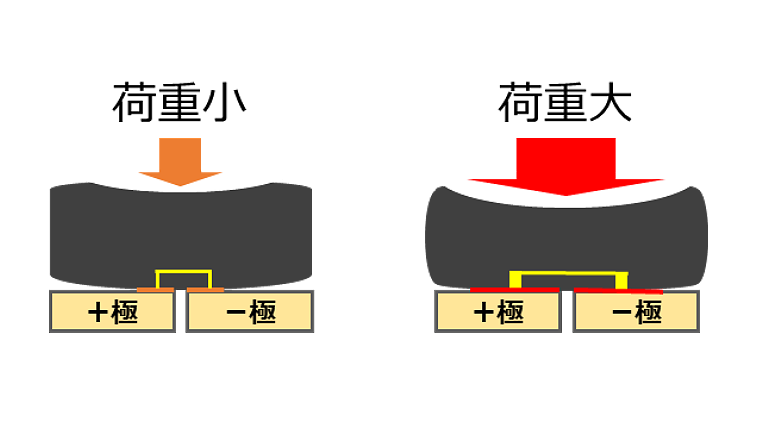
\includegraphics[scale=0.45]{/Users/ohyamasan/Downloads/TMCIT-Report/EE_Measurement/fig/sensor-03.png}
\caption{力センサの原理}
\label{fig:weight}
\end{figure}

\subsection{発光ダイオード\cite{dafadsav}\cite{gjkdgfbn}}
\label{LEDG}
LED(Light Emitting Diode)ともいう.
pn接合でできている.順方向の電圧を加えることにより,再結合エネルギーが光になって放出される.
電気エネルギーを直接光エネルギーに変換できるため,従来の光源と比べてエネルギー効率が高い.
白色LEDは\wfig{aokiro}のように,青色LED+黄色蛍光体(現在主流)のものと,\wfig{rgb}のように,赤色LED+緑色LED+青色LEDで作るものなどがある.

\begin{figure}[h]
  \begin{minipage}[]{0.5\hsize}
    \centering
    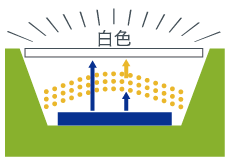
\includegraphics[scale=0.8]{/Users/ohyamasan/Downloads/TMCIT-Report/EE_Measurement/fig/led_what3_jp1.png}
    \caption{青色+黄色蛍光体手法}
    \label{fig:aokiro}
  \end{minipage}
  \begin{minipage}[]{0.5\hsize}
    \centering
    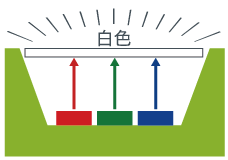
\includegraphics[scale=0.8]{/Users/ohyamasan/Downloads/TMCIT-Report/EE_Measurement/fig/led_what3_jp2.png}
    \caption{赤色+緑色+青色手法}
    \label{fig:rgb}
  \end{minipage}
\end{figure}


\subsection{真値と誤差及び相対誤差(誤差率)\cite{1130000797667922816}}
\subsubsection{真値(true value)}
真値とは,測定量(測定値ではない)が単位の何倍であるのかを示している値である.
真値は必ず存在すると仮定しても我々は真値そのものは知ることができず,ただその存在する範囲を推定することが出来るだけである.
そのため誤差は正負の符号を持っているが,それを確定することができない.
\subsubsection{誤差及び相対誤差}
測定値(measured value)及び,誤差(error)はそれぞれ,\weq{keisoku},\weq{gosa}で定義される.
\begin{align}
	測定値 &= 倍数 \times 単位\label{eq:keisoku}\\
	誤差 &= 測定値 − 真値\label{eq:gosa}
\end{align}
また,相対誤差(relative error)とは真値に対する誤差の比である.
但し真値は不明なことが多いため,通常は\weq{soutaigosa}のように誤差が小さいとして真値の代わりに測定値で割る.
\begin{eqnarray}
	相対誤差 = \frac{誤差}{真値} \fallingdotseq \frac{誤差}{測定値}
	\label{eq:soutaigosa}
\end{eqnarray}
相対誤差を百分率などで表した値を誤差率と呼ぶ.
また,以上のことから\weq{hutasikasa}のように表すこともできることがわかる\cite{1130000797042387712}.
\begin{eqnarray}
	測定値=真値 \pm 誤差=真値(1\pm 相対誤差)
\label{eq:hutasikasa}
\end{eqnarray}

\subsection{統計処理(正規分布・平均値・標準偏差)}
\subsubsection{正規分布(normal distribution)\cite{1130848328216058496}\cite{6602}}
左右対称の釣鐘型(平均値から離れるにつれて個数が減る)に値が分布している分布で,山の頂点に平均値がくる.
\wfig{normal-fig}は横軸に測定量,縦軸に正規分布の確率密度関数(probability density function)をプロットしたものである.
全体の面積(全確率)は\weq{int-nor}より1である.

\begin{figure}
\centering
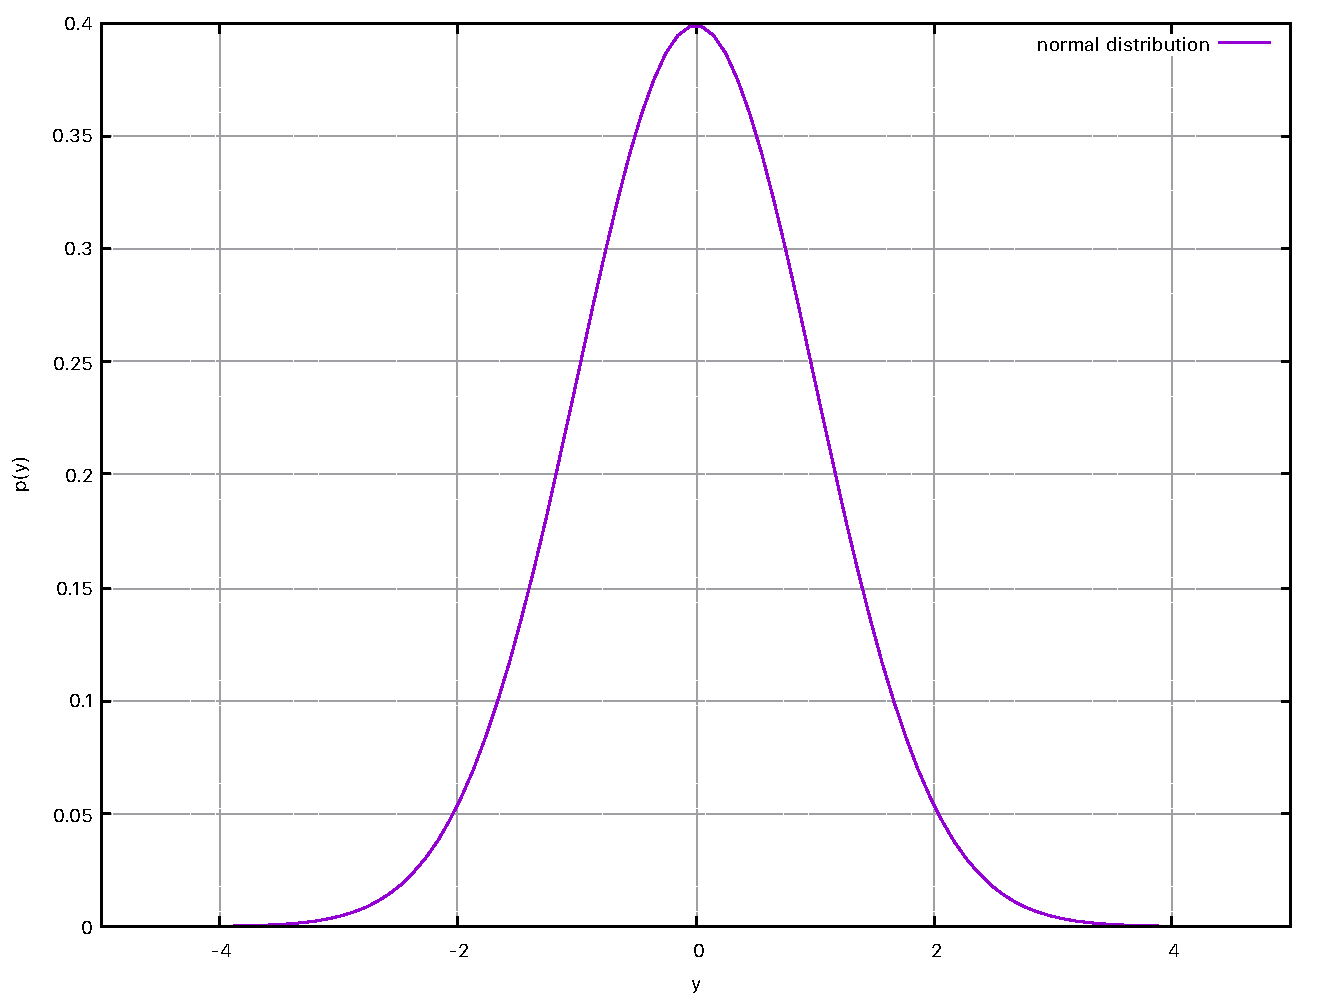
\includegraphics[scale=0.5]{/Users/ohyamasan/Downloads/TMCIT-Report/EE_Measurement/pre/plot.pdf}
\caption{正規分布}
\label{fig:normal-fig}
\end{figure}

\begin{equation}
\label{13}
p(x)=p(X=x)
\end{equation}

\begin{equation}
\label{eq:kakuritumitudo-fx}
p(x)=\frac{1}{\sqrt{2\pi}\sigma} \exp \left\{-\frac{(x-\mu)^2}{2\sigma^2}\right\}
\end{equation}

\begin{align}
\label{eq:int-nor}
\int_{-\infty}^{\infty} p(x)\,dx&=\frac{1}{\sqrt{2\pi}\sigma} \int_{-\infty}^{\infty} \exp \left(\frac{(x-\mu)^{2}}{2\sigma^{2}}\right)dx\nonumber\\
=&\frac{1}{\sqrt{2\pi}\sigma } \int_{-\infty}^{\infty} \exp \left(-\frac{y^{2}}{2\sigma^{2}}\right)dy\nonumber\\
=&\frac{1}{\sqrt{2\pi}\sigma }\sqrt{2\sigma^{2}\pi}=1
\end{align}

\subsubsection{平均値(mean)}
(算術)平均値とは$N$個全てのデータの総和を$N$個で割って得られる値で,\weq{heikinchi}で表すことができる\cite{1130848328216058496}.
\begin{equation}
	\bar{y} = \frac{1}{N}\sum^N_{i = 1}y_i
	\label{eq:heikinchi}
\end{equation}		

\subsubsection{標準偏差(standard deviation)\cite{1130000797042387712}}
標準偏差とは平均値を基準に各測定量がどれほどのばらついているかを定量的に表す値で,\weq{hyoujunhensa}で表すことができる.
\begin{equation}
	\sigma = \sqrt{\frac{1}{N - 1}\sum^N_{i = 1}(y_i - \bar{y})^2}
	\label{eq:hyoujunhensa}
\end{equation}	

\subsection{最小二乗法(method of least squares)\cite{1130848328216058496}\cite{1130282272174486912}}
2つの測定データ$y, x$間に一次方程式の関係があるとし,
\begin{equation}
	y = ax + b
	\label{eq:aiu}
\end{equation}
の傾き$a$,切片$b$を測定データからもっともらしい値にすることを考える.
その際に,
\begin{eqnarray}
	I &=& \sum\limits_{i=1}^{N} \varepsilon^2_i \nonumber\\
	&=& \sum\limits_{i=1}^{N} \bigl( y_i - f(x_i)\bigr)^2\nonumber\\\
	&=& \sum\limits_{i=1}^{N} \bigl( y_i - (ax_i+b)\bigr)^2
	\label{eq:error}
\end{eqnarray}
を最小にする$a$,$b$を求める.
これを最小二乗法といい,誤差を伴う測定値の処理においてその誤差の二乗の和を最小にすることで,最も確からしい関係式を求める方法である.前述の通り,誤差は正負あるため,2乘をしている.絶対値を用いると偏微分が不可能なため,平方根を用いた方法で行っている.
\begin{eqnarray}
	\frac{\partial}{\partial a}I(a,b) &=& 0\\
	\frac{\partial}{\partial b}I(a,b) &=& 0
\end{eqnarray}
から得られる方程式を,それぞれ$a$,$b$について解けば良く,それぞれの解を得るための方程式は次の2つを用いることになる.
\begin{equation}
	a = \frac{\sum_{n=1}^{n}(x_i -\bar{x})(y_i-\bar{y})}{\sum_{n=1}^{n}(x_i-\bar{x})^2}
	\label{eq:saisyou1}
\end{equation}
\begin{equation}
	b = \bar{y}-\frac{\sum_{n=1}^{n}(x_i -\bar{x})(y_i-\bar{y})}{\sum_{n=1}^{n}(x_i-\bar{x})^2} \bar{x}
	\label{eq:saisyou2}
\end{equation}
ここでは,\weq{aiu}のように1次式の形のものを示したが,一般に\weq{ippan}のような実験式に対して\weq{least-i}のように定義される.
\begin{align}
y&=F(x;a,b,c,\cdots)\label{eq:ippan}\\
(&xは変数,a,b,c,\cdots は定数)\nonumber
\end{align}
\begin{equation}
\label{eq:least-i}
I \equiv \sum_{i} (y_{i}-f(x_{i}))^{2} \quad \left(\frac{\partial I}{\partial a}=0 \to aを決定,\frac{\partial I}{\partial b}=0 \to bを決定 \cdots \right)
\end{equation}



\section{ダイオードの特性実験}
\subsection{使用器具}
	ダイオードの特性実験の使用機材を以下の\wtab{diode_apparatus}に示す。

	\begin{table}[hbt]
		\centering
		\caption{使用器具}
		\begin{tabular}{|c||c|c|c|} \hline
				使用器具名 & 製造元 & 型番 & 製造番号(管理番号)\\ \hline
				電流計(ミリアンペア計) & YOKOGAWA & E-CLASS 1.0 & 48-2 \\ \hline
				電圧計 & YOKOGAWA & E-CLASS 1.0 & 278-20 \\ \hline
				電源装置 & YOKOGAWA & PA1811 & L69-000668 \\ \hline
		\end{tabular}
		\label{tab:diode_apparatus}
	\end{table}

% % % % % % % % % % % % % % % % % % % % % % % % % % % % % % % % % % % % % % % % % % % % % % % % % % % % % % 
\subsection{順バイアス}
\subsubsection{実験方法}
  順バイアスのダイオードの特性計測に用いた回路を\wfig{diode1_circuit} に示す。

  \begin{figure}[!h]
    \centering
    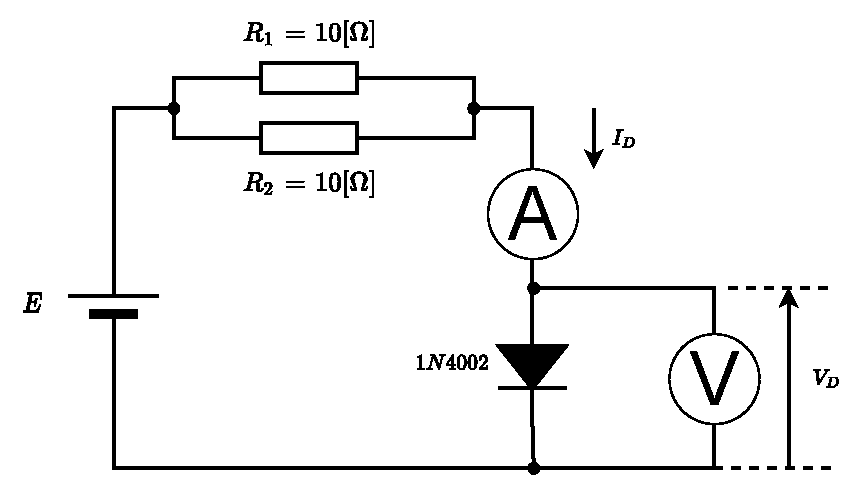
\includegraphics[width=10cm]{./pdfs/diode1.pdf}
    \caption{順バイアスのダイオードの回路図}
    \label{fig:diode1_circuit}
  \end{figure}

  この実験では直流電源Eの電圧を0.0~0.8 V まで0.1 V ずつ増加させた。
  そのときの電圧$V_D$,電流$I_D$を計測した。
  また,必要に応じて計測点を増やした。

\subsubsection{結果}
  計測して得られたデータを\wtab{diode1_result} に示す。
  また,\wtab{diode1_result} から作成したグラフを\wfig{forward_bias_ID-VD} に示す。
  このグラフから,順バイアスのときダイオードにかかる電圧が0.6 V 以上の場合,電流を通すことが分かる。
  また,0.6 V 以下の場合ほとんど電流を通さないことも分かる。
  約0.7 V から通す電流が著しく増加していることが分かる。

  \begin{table}[hbt]
    \centering
    \caption{順バイアスのダイオード特性の測定結果}
    \begin{tabular}{|c|c|} \hline
        電圧 & 電流 \\
        $V_D$ [V] & $I_D$ [mA] \\ \hline
        0.000 & 0.0 \\ \hline
        0.100 & 0.0 \\ \hline
        0.200 & 0.0 \\ \hline
        0.300 & 0.0 \\ \hline
        0.400 & 0.0 \\ \hline
        0.500 & 0.0 \\ \hline
        0.600 & 0.5 \\ \hline
        0.648 & 5.0 \\ \hline
        0.678 & 10.0 \\ \hline
        0.700 & 17.5 \\ \hline
        0.722 & 30.0 \\ \hline
        0.746 & 50.0 \\ \hline
        0.760 & 75.0 \\ \hline
        0.770 & 100.0 \\ \hline
        0.788 & 150.0 \\ \hline
        0.800 & 182.5 \\ \hline
    \end{tabular}
    \label{tab:diode1_result}
  \end{table}

  \begin{figure}[!h]
    \centering
    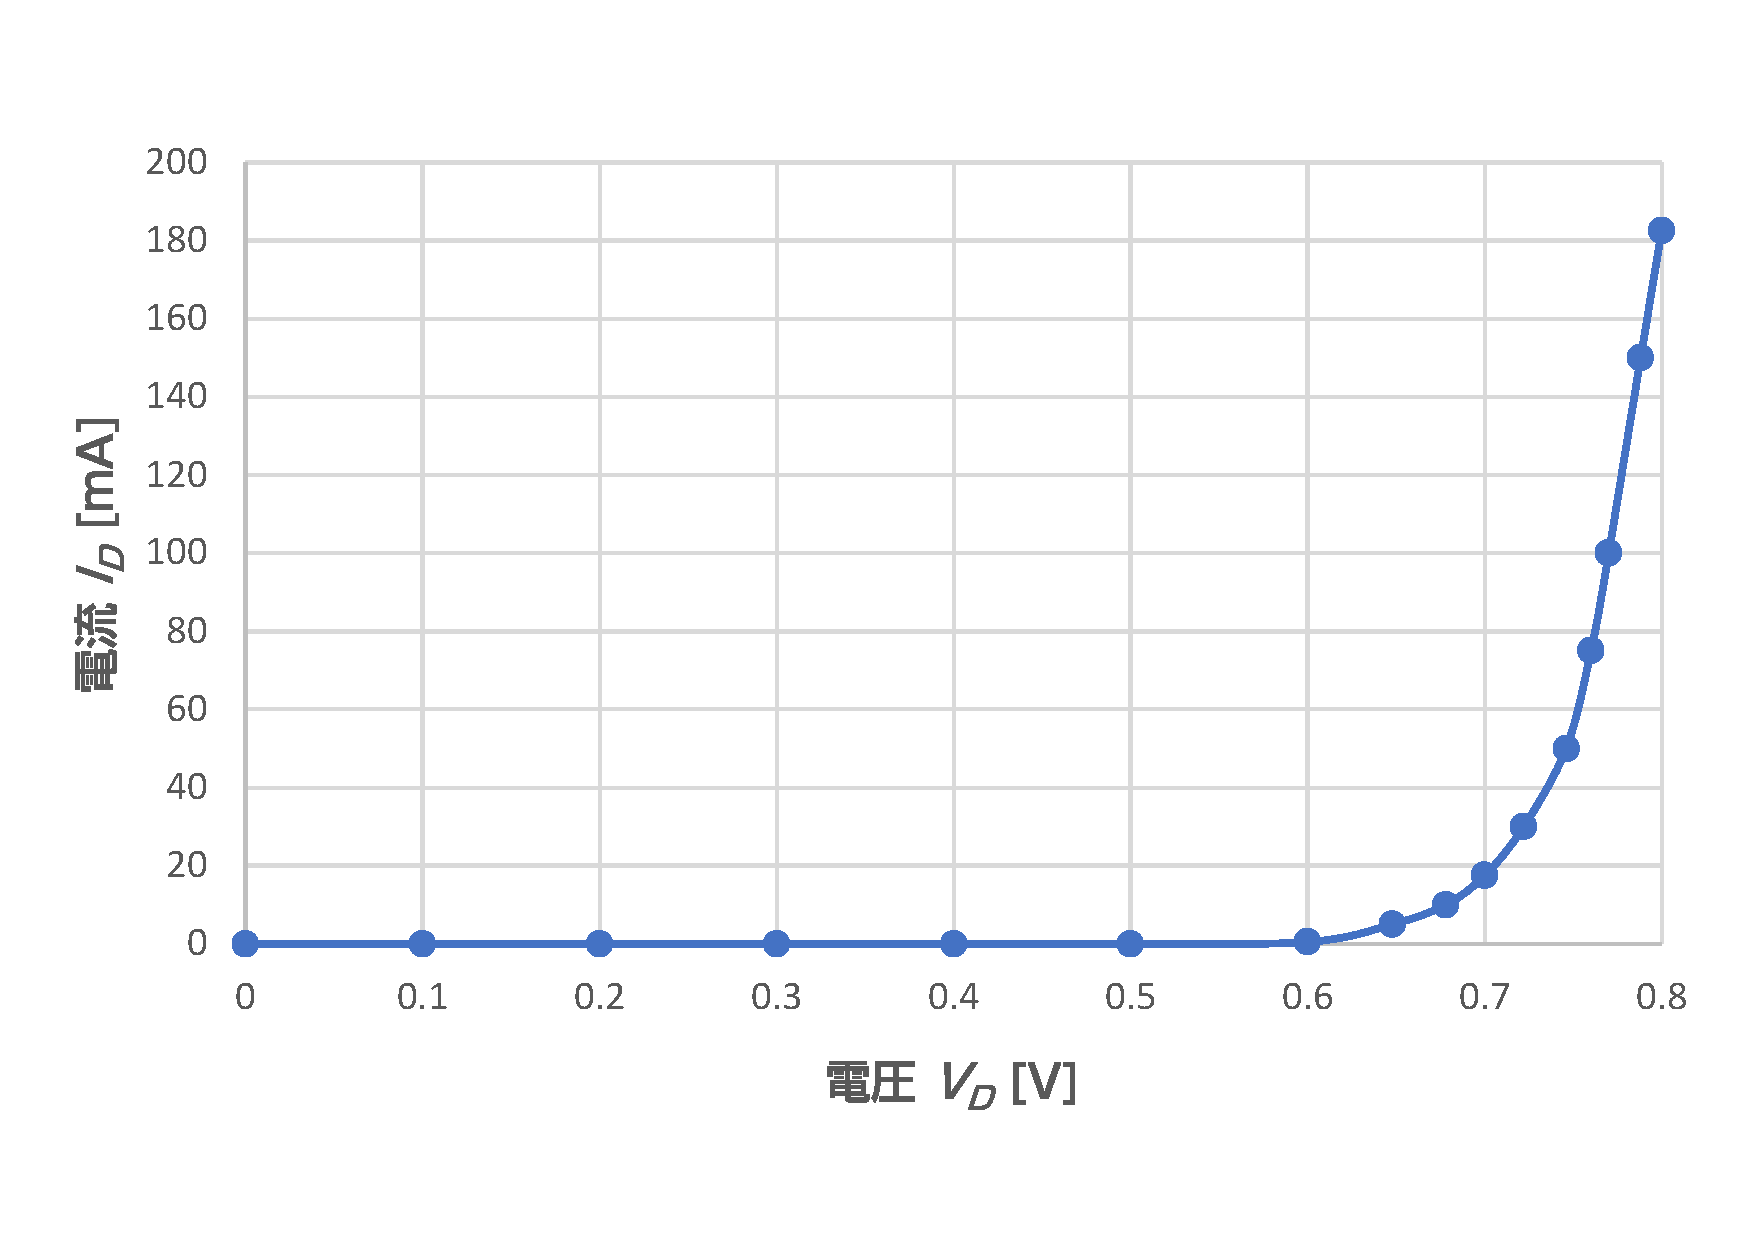
\includegraphics[width=13cm]{./figs/G-forward_bias_ID-VD.pdf}
    \caption{順バイアスのダイオードの電圧電流特性}
    \label{fig:forward_bias_ID-VD}
  \end{figure}

\newpage%%%%%
\subsubsection{考察}
  直流電圧電流特性グラフを説明せよ。\\

  \begin{figure}[!h]
    \centering
    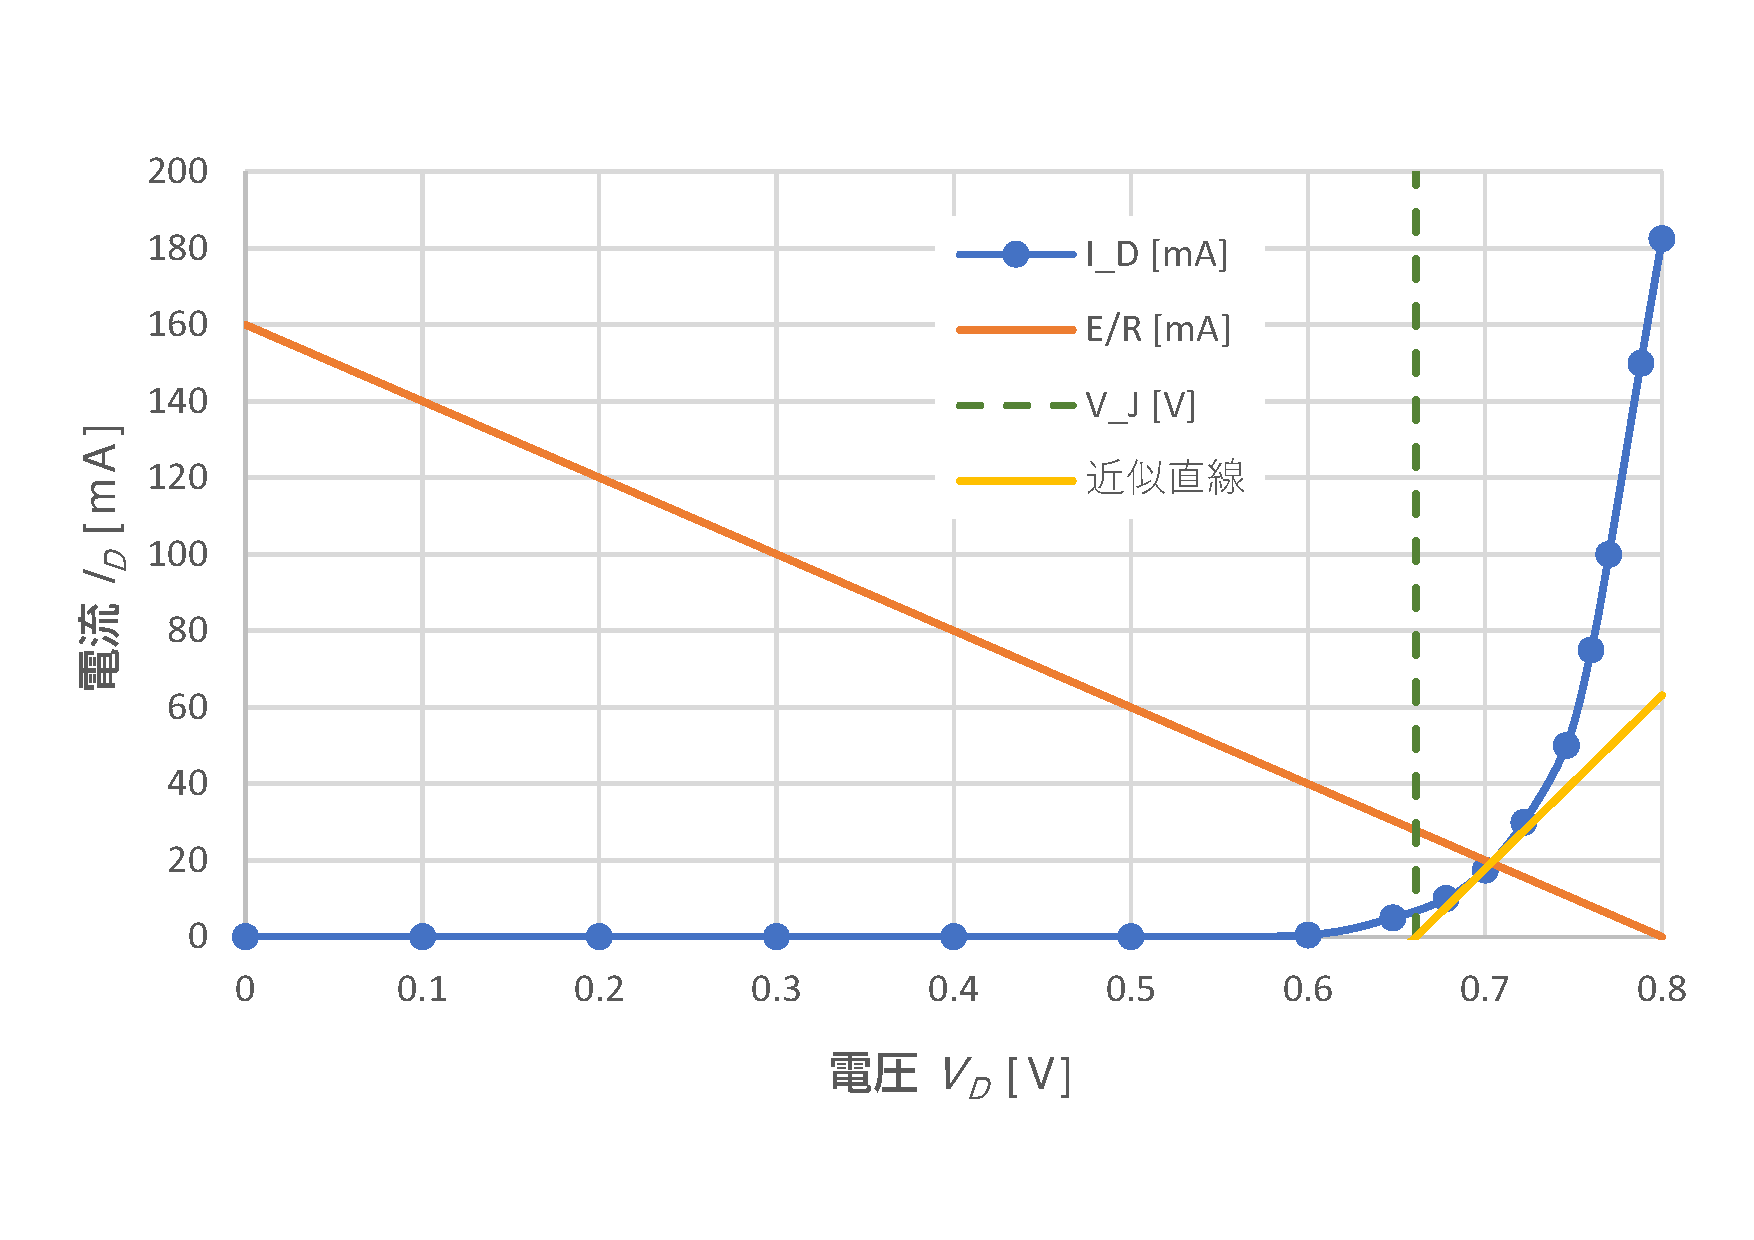
\includegraphics[width=13cm]{./figs/G-forward_discussion.pdf}
    \caption{順バイアス電流と負荷線と立ち上がり電圧}
    \label{fig:forward_discussion}
  \end{figure}
  
  \begin{table}[hbt]
    \centering
    \caption{tab:順バイアスの測定結果と負荷線と誤差}
    \begin{tabular}{|c|c|c|c|}
    \hline
    電圧 & 電流 & 電流 & 電流(誤差) \\
    $V_D$ [V] & $I_D$ [mA] & $E/R$ [mA] & $|I_D-E/R|$ [mA] \\ \hline
    0            & 0             & 160          & 160                 \\ \hline
    0.1          & 0             & 140          & 140                 \\ \hline
    0.2          & 0             & 120          & 120                 \\ \hline
    0.3          & 0             & 100          & 100                 \\ \hline
    0.4          & 0             & 80           & 80                  \\ \hline
    0.5          & 0             & 60           & 60                  \\ \hline
    0.6          & 0.5           & 40           & 39.5                \\ \hline
    0.648        & 5             & 30.4         & 25.4                \\ \hline
    0.678        & 10            & 24.4         & 14.4                \\ \hline
    0.7          & 17.5          & 20           & 2.5                 \\ \hline
    0.722        & 30            & 15.6         & 14.4                \\ \hline
    0.746        & 50            & 10.8         & 39.2                \\ \hline
    0.76         & 75            & 8            & 67                  \\ \hline
    0.77         & 100           & 6            & 94                  \\ \hline
    0.788        & 150           & 2.4          & 147.6               \\ \hline
    0.8          & 182.5         & 0            & 182.5               \\ \hline
    \end{tabular}
    \label{tab:diode1_}
  \end{table}

  \wfig{forward_discussion} は\wfig{forward_bias_ID-VD} に負荷線,接線の近似直線,立ち上がり電圧を追記したものだ。
  負荷線は$\frac{V_R}{R}$で計算した。
  $V_R$は抵抗にかかっている電圧であり,分圧則\cite{tyosho:denkiKiso1}より$V_R = E - V_D$($E=0.8\mathrm{[V]}$)と計算した。
  $R$は$R_1$と$R_2$の合成抵抗と考え,\weq{resistance_calc} のように計算した。
  よって,合成抵抗$R=5[\Omega]$ である。
  \begin{align}
    R &= \frac{R_1*R_2}{R_1 + R_2} \nonumber \\
    &= \frac{10*10}{10 + 10} \nonumber \\
    &= 5 \label{eq:resistance_calc}
  \end{align}
  接線の近似直線は以下の手順で求めた。
  \begin{enumerate}
    \item $I_D$と$E/R$の誤差を計算する。
    \item $V_D = 0.7 \mathrm{[V]}$で最も誤差が小さくなっているので,$V_D = 0.7 \mathrm{[V]}$に近い前後2点から傾きを計算する。
        \begin{align}
          \begin{cases}
            dV_D &= 0.722 - 0.678 \nonumber \\
            &= 0.044 \mathrm{[V]} \nonumber \\
            dI_D &= 30 - 10 \nonumber \\
            &= 20 \mathrm{[mA]} \nonumber \\
          \end{cases} \nonumber \\
          \frac{dI_D}{dV_D} &= \frac{20}{0.044} \nonumber \\
          &\approx 454.5 \label{eq:approxLine_calc}
        \end{align}
    \item 以下の式に$V_D = 0.7 \mathrm{[V]}$のときの値を代入し,$V_J$(x切片)を計算する。
        \begin{align}
          I_D &= \frac{dI_D}{dV_D} (V_D - V_J) \nonumber \\
          \begin{cases}
            \frac{dI_D}{dV_D} &= 454.5 \nonumber \\
            V_D &= 0.700 \nonumber \\
            I_D &= 17.5 \nonumber \\
          \end{cases} \nonumber \\
          17.5 &= 454.5(0.700 - V_J) \nonumber \\
          V_J &\approx 0.661 \mathrm{[V]} \nonumber
        \end{align}
    \item よって下式が接線の近似直線の式である。
        \begin{equation}
          I = 454.5 (V - 0.661) \mathrm{[mA]} \label{eq:approxLine}
        \end{equation}
  \end{enumerate}
  立ち上がり電圧は接線の近似直線と$I = 0 \mathrm{[mA]}$の交点である。
  $I = 0 \mathrm{[mA]}$を\weq{approxLine} に代入すると,V = 0.661 [V] である。
  よって,立ち上がり電圧は 0.661 V である。

  微分抵抗$r_d$は\weq{approxLine_calc} の$\frac{dI_D}{dV_D}$の分母と分子を入れ替えることで計算できる。
  よって$r_d$は以下のようにして求めれられる。
  \begin{equation}
    r_d = \frac{dI_D}{dV_D} = \frac{0.044}{20*10^{-3}} = 2.2 \mathrm{[\Omega]} \nonumber
  \end{equation}
  
  \wfig{risou1} は$r_d$,$V_J$,理想ダイオードで構成された等価回路である。
  $r_d$はダイオードの抵抗成分を示し,$V_J$はダイオードの内部で発生する電界から生まれる電圧降下を示す。
  理想ダイオードはダイオードの整流作用を示す。
  \begin{figure}[!h]
    \centering
    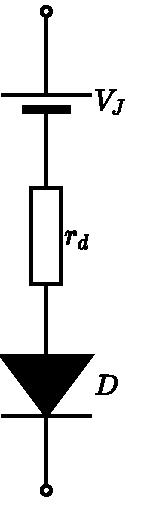
\includegraphics[width=2cm]{./pdfs/risou1.pdf}
    \caption{順バイアスのダイオードの等価回路}
    \label{fig:risou1}
  \end{figure}

% % % % % % % % % % % % % % % % % % % % % % % % % % % % % % % % % % % % % % % % % % % % % % % % % % % % % % 
\subsection{逆バイアス}
\subsubsection{実験方法}
  逆バイアスのダイオードの特性計測に用いた回路を\wfig{diode2_circuit} に示す。

  \begin{figure}[!h]
    \centering
    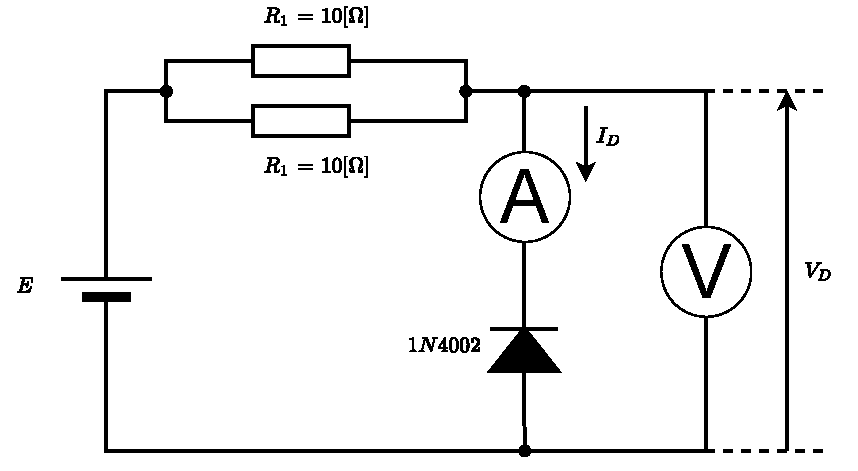
\includegraphics[width=10cm]{./pdfs/diode2.pdf}
    \caption{逆バイアスのダイオードの回路図}
    \label{fig:diode2_circuit}
  \end{figure}

  この実験では直流電源Eの電圧を0~8 V まで1 V ずつ増加させた。
  そのときの電圧$V_D$,電流$I_D$を計測した。

\subsubsection{結果}
  計測して得られたデータを\wtab{diode1_result} に示す。
  また,\wtab{diode1_result} から作成したグラフを\wfig{reverse_bias_ID-VD} に示す。
  このグラフから,逆バイアスのときダイオードにかかる電圧が8 V になっても,ダイオードは電流を通さないことが分かる。
  また,\wfig{forward_bias_ID-VD} と比べて,非常に高い電圧になっても電流を通さないことも分かる。
  このことから,ダイオードの整流作用\cite{tyosho:densiKairo} を確認できる。

  \begin{table}[hbt]
    \centering
    \caption{逆バイアスのダイオード特性の測定結果}
    \begin{tabular}{|c|c|} \hline
        電圧 & 電流 \\
        $V_D$ [V] & $I_D$ [mA] \\ \hline
        0 & 0 \\ \hline
        1 & 0 \\ \hline
        2 & 0 \\ \hline
        3 & 0 \\ \hline
        4 & 0 \\ \hline
        5 & 0 \\ \hline
        6 & 0 \\ \hline
        7 & 0 \\ \hline
        8 & 0 \\ \hline
    \end{tabular}
    \label{tab:diode2_result}
  \end{table}

  \begin{figure}[!h]
    \centering
    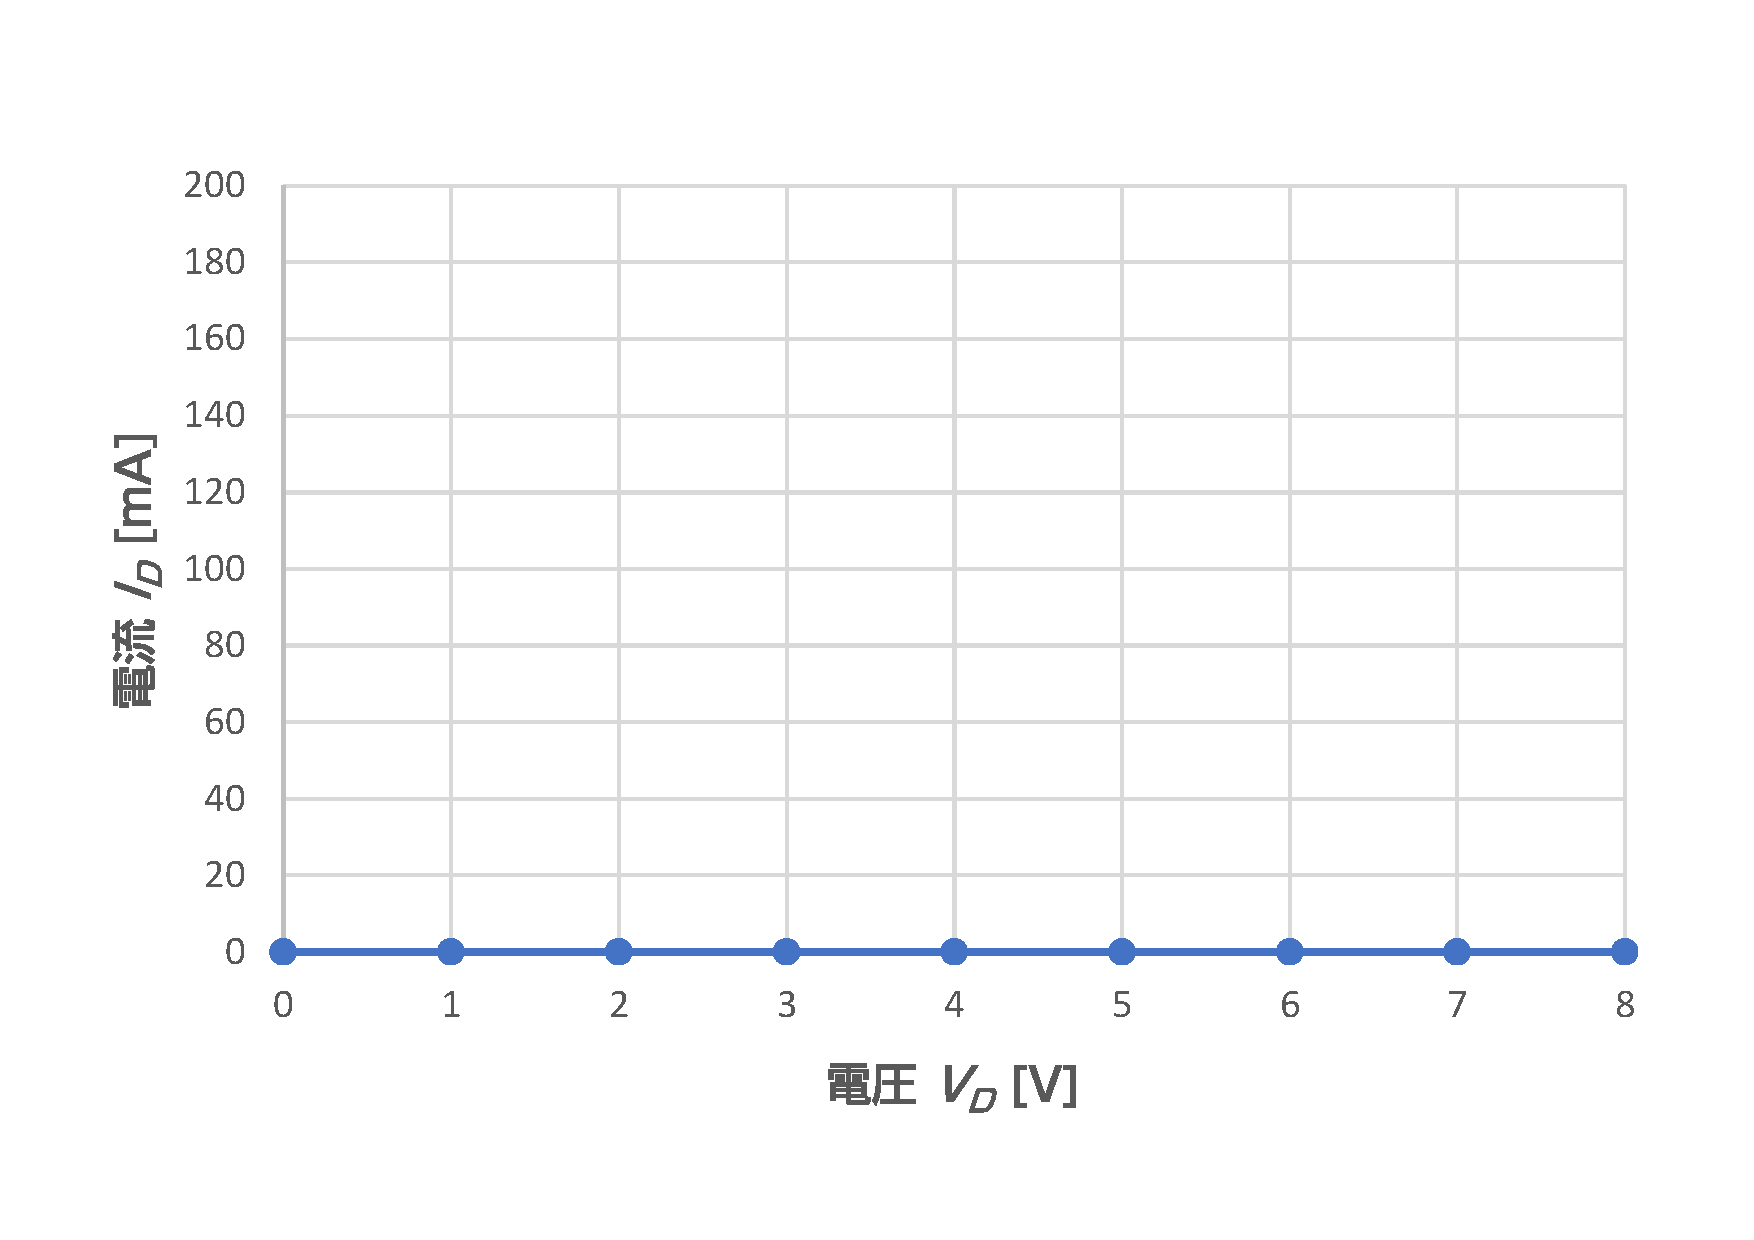
\includegraphics[width=8.2cm]{./figs/G-reverse_bias_ID-VD}
    \caption{逆バイアスのダイオードの電圧電流特性}
    \label{fig:reverse_bias_ID-VD}
  \end{figure}

\subsubsection{考察}
  実験で用いたダイオードのデータシートから逆方向電流の値を調べよ。
  また,逆バイアスの場合でもわずかに電流が流れる理由を図を用いて説明せよ。

  1N4001のデータシート\cite{web:1N4001} によると,ダイオード1N4002は逆バイアス時に 5 uA のドリフト電流を流す。
  ダイオードに逆バイアスをかけたとき,  n型p型ともに多数キャリアが再結合で減少する。
  また,同時に少数キャリアが移動する。
  このときの少数の電子の移動によりドリフト電流が流れる。
  \wfig{2} では多数キャリアに注目しているので,電子は移動せず電流は流れないように考えられる。
  しかし,p型半導体の少数キャリアの電子が移動するため,僅かに電流は流れてしまう。

\newpage
\section{ツェナーダイオードの特性実験}
\subsection{使用器具}
	ツェナーダイオードの特性実験の使用機材を以下の\wtab{zenerDiode_apparatus}に示す。
	\begin{table}[hbt]
		\centering
		\caption{使用器具}
		\begin{tabular}{|c||c|c|c|} \hline
				使用器具名 & 製造元 & 型番 & 製造番号(管理番号)\\ \hline
				電流計(ミリアンペア計)1 & YOKOGAWA & E-CLASS 1.0 & 48-2 \\ \hline
				電流計(ミリアンペア計)2 & YOKOGAWA & E-CLASS 1.0 & 578 \\ \hline
				電圧計 & YOKOGAWA & E-CLASS 1.0 & 278-20 \\ \hline
				電源装置 & YOKOGAWA & PA1811 & L69-000668 \\ \hline
				可変抵抗3 & TOKUSHU DENKI KOGYOSHO & S-3 & 3201 \\ \hline
		\end{tabular}
		\label{tab:zenerDiode_apparatus}
	\end{table}

%	% %	%	%	% %	% %	%	%	% %	% %	%	%	% %	% %	%	%	% %	% %	%	%	% %	% %	%	%	% %	% %	%	%	%
\subsection{ツェナーダイオードの特性}
\subsubsection{実験方法}
	ツェナーダイオードの特性計測に用いた回路を\wfig{zenerDiode1_circuit} に示す。

	\begin{figure}[!h]
    \centering
    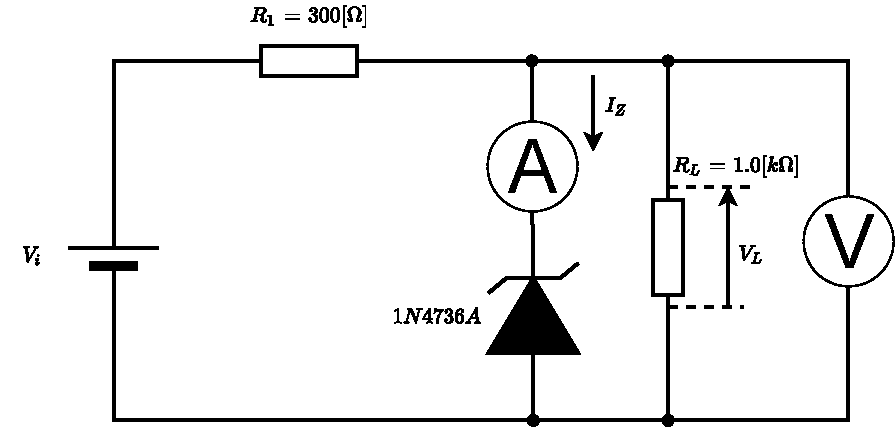
\includegraphics[width=10cm]{./pdfs/zener_diode1.pdf}
    \caption{ツェナーダイオード特性の回路図}
    \label{fig:zenerDiode1_circuit}
  \end{figure}
	
  この実験では直流電源の電圧$V_i$を18~0 V まで1 V ずつ減少させた。
  そのときの電流$I_Z$,電圧$V_L$を計測した。

\subsubsection{結果}
	計測して得られたデータを\wtab{zenerDiode1_result} に示す。
	また\wtab{zenerDiode1_result} から作成したグラフを\wfig{zener_Vi-VLIZ} に示す。
	この表から,入力電圧$V_i$が0~8 V ではツェナーダイオードに電流が流れていないことが分かる。
	電圧$V_L$は,ツェナーダイオードと並列に接続されている抵抗の電圧であり,ツェナーダイオードの電圧$V_D$でもある。
	電圧$V_L$が6.61 V のとき,ツェナーダイオードは電流を流し始めている。
	その後,入力電圧$V_i$が増加しても,$V_L$はあまり変化していないことが分かる。
	また,$V_L$の変化が減ると同時に,ツェナーダイオードに流れる電流$I_Z$が増加していることが分かる。

	\begin{table}[hbt]
		\centering
		\caption{ツェナーダイオードの特性の計測結果}
		\begin{tabular}{|c|c|c|}
		\hline
		電圧$V_i$ [V] & 電圧$V_L$ [V] & 電流$I_Z$ [mA] 			 \\ \hline
		0            & 0            & 0             \\ \hline
		1            & 0.78         & 0             \\ \hline
		2            & 1.54         & 0             \\ \hline
		3            & 2.28         & 0             \\ \hline
		4            & 3.06         & 0             \\ \hline
		5            & 3.82         & 0             \\ \hline
		6            & 4.58         & 0             \\ \hline
		7            & 5.35         & 0             \\ \hline
		8            & 6.1          & 0             \\ \hline
		9            & 6.61         & 1             \\ \hline
		10           & 6.64         & 4.2           \\ \hline
		11           & 6.66         & 7.8           \\ \hline
		12           & 6.69         & 10.8          \\ \hline
		13           & 6.72         & 16.2          \\ \hline
		14           & 6.74         & 17.6          \\ \hline
		15           & 6.76         & 20.8          \\ \hline
		16           & 6.78         & 24.2          \\ \hline
		17           & 6.8          & 27.8          \\ \hline
		18           & 6.82         & 30.8          \\ \hline
		\end{tabular}
		\label{tab:zenerDiode1_result}
	\end{table}

	\begin{figure}[!h]
    \centering
    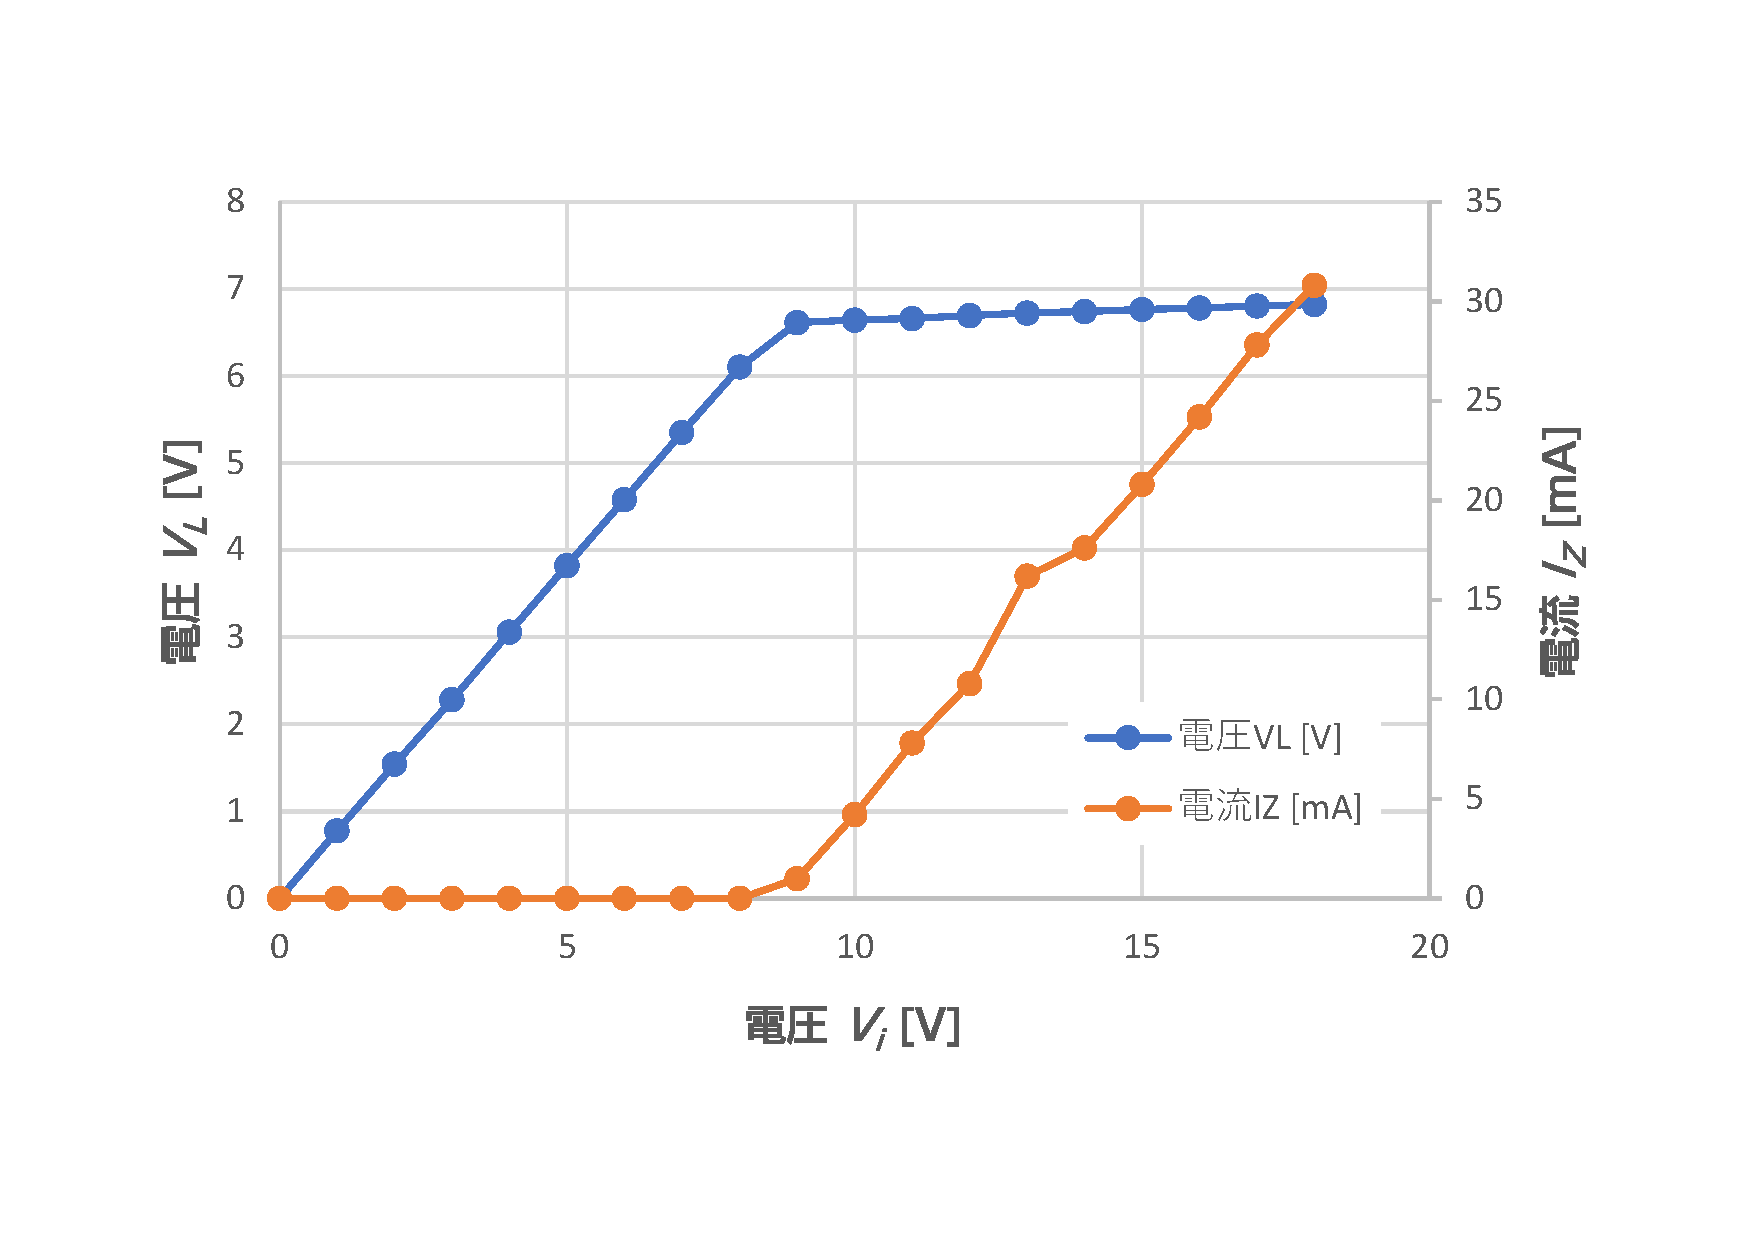
\includegraphics[width=13cm]{./figs/G-zener_Vi-VLIZ.pdf}
    \caption{入力電圧とツェナーダイオードの電圧電流特性}
    \label{fig:zener_Vi-VLIZ}
  \end{figure}

\subsubsection{考察}
	\begin{enumerate}
		\item ツェナーダイオード 1N4736A のデータシートでツェナー電圧を調べ,実験結果と比較して考察せ
		よ。\\

		1N4736A のデータシート\cite{web:1N4736A} によると, ツェナーダイオード 1N4736A のツェナー電圧は Typ. 6.8 V (25℃)である。
		\wtab{zenerDiode1_result} より,$V_L$が6.61~6.82 V の間でツェナーダイオードに電流が流れていることが分かる。
		電流が流れている間の$V_L$の平均値は 6.72 V である。
		データシートの値と計測値にほとんど差がなく,計測が成功していると考えられる。

		\item ツェナーダイオードはどのような場合に用いられるか説明せよ。\\
  
		ツェナーダイオードは一定電圧を保つダイオードである。
		マイクロマウスなどのロボットは,壁やラインを検知するために,フォトリフレクタを用いる。
		フォトリフレクタは,LEDとフォトダイオード(フォトトランジスタ)で構成される。
		LEDを発光させ,反射光をフォトダイオードで強度から,距離や色を検知するものである。
		このとき,LEDの出力が一定でないと正確なデータを計測できず,ロボットがパフォーマンスを発揮しきれないことがある。
		そこで,ツェナーダイオード用いることで,各LEDにかかる電圧を一定にでき,LEDの出力を安定化させることができる。

  	\item VL − VZ 特性のグラフを書き,ツェナー電圧 VZ を説明せよ。\\
   
		\wfig{zener_VL-IZ} はツェナーダイオードの電圧電流特性とツェナー電圧を示したグラフである。
		ツェナー電圧は $V_L = $6.8 V と設定した。
		ツェナー電圧とツェナーダイオードの電圧電流特性のグラフはほとんど一致している。
		このことから,このツェナーダイオードのツェナー電圧は約6.8 V だと考えられる。
   
		\begin{figure}[!h]
			\centering
			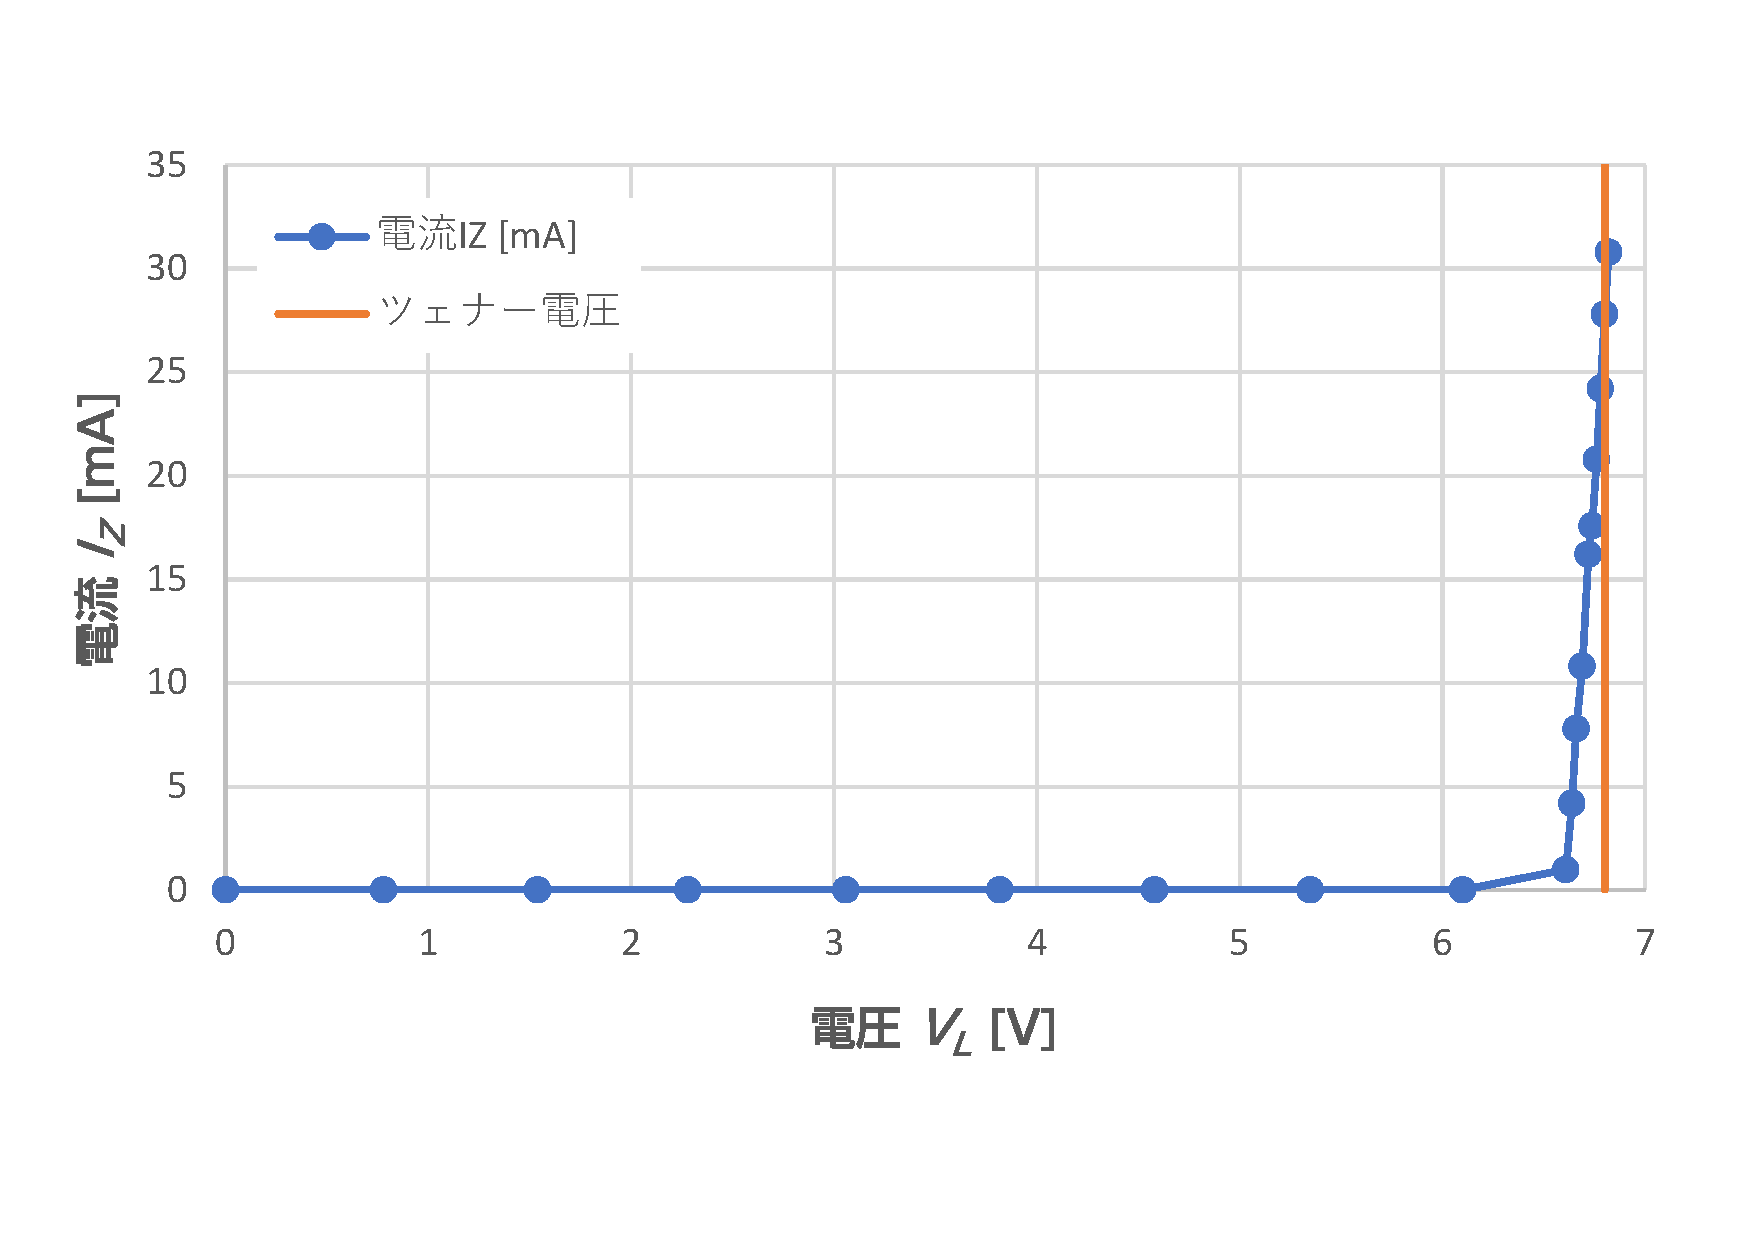
\includegraphics[width=13cm]{./figs/G-zener_VL-IZ.pdf}
			\caption{ツェナーダイオードの電圧電流特性とツェナー電圧}
			\label{fig:zener_VL-IZ}
		\end{figure}

   	\item 各グラフから入出力特性を考察せよ。\\
     
		\wfig{zener_VL-IZ} より,ツェナーダイオードは一定電圧を超えると,急激に電流を通すようになる特性が考えられる。
		また,急激に電流を通すようになることから,急激に抵抗値が低下しているとも考えられる。
		\wfig{zener_Vi-VLIZ} より,ツェナーダイオードは一定電圧を保つ特性があると考えられる。
		
	\end{enumerate}

%	% %	%	%	% %	% %	%	%	% %	% %	%	%	% %	% %	%	%	% %	% %	%	%	% %	% %	%	%	% %	% %	%	%	%
\subsection{ツェナーダイオード定電圧回路}
\subsubsection{実験方法}
	ツェナーダイオード定電圧特性の計測に用いた回路を\wfig{zenerDiode2_circuit} に示す。

	\begin{figure}[!h]
		\centering
		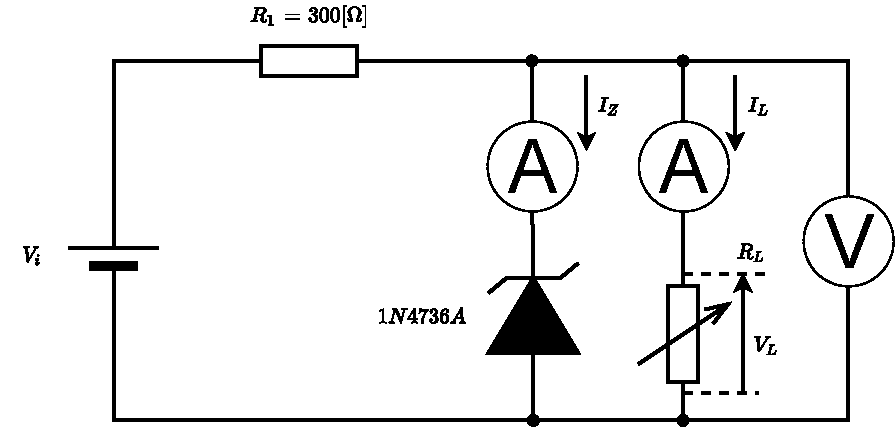
\includegraphics[width=10cm]{./pdfs/zener_diode2.pdf}
		\caption{ツェナーダイオード定電圧特性の回路図}
		\label{fig:zenerDiode2_circuit}
	\end{figure}

	この実験では直流電源の電圧$V_i$を15 V に固定し,可変抵抗$R_L$を変化させて,ツェナー電流$I_Z$が2~22 mA まで2 mA ずつ増加するようにした。
	そのときの出力電圧$V_L$,出力電流$I_L$を計測した。

\subsubsection{結果}
	計測して得られたデータを\wtab{zenerDiode2_result} に示す。
	また\wtab{zenerDiode2_result} から作成したグラフを\wfig{zener_IZ-VL} と\wfig{zener_IZ-IL} に示す。
	\wfig{zener_IZ-VL} から,ツェナー電流$I_Z$に関わらず,ツェナー電圧$V_Z$はほとんど一定であることが分かる。
	\wfig{zener_IZ-IL} から,ツェナー電流$I_Z$が増加すると,$I_L$が減少していることが分かる。
	また,$I_L$は$I_Z$に比例して減少していることも分かる。

	\begin{table}[hbt]
		\centering
		\caption{ツェナーダイオードの定電圧特性の計測結果}
		\begin{tabular}{|c|c|c|}
		\hline
		電流$I_Z$ [mA] & 電流$I_L$ [mA] & 電圧$V_L$ [V] \\ \hline
		2                        & 25.85           & 6.6            \\ \hline
		4                        & 23.9            & 6.62           \\ \hline
		6                        & 21.9            & 6.62           \\ \hline
		8                        & 19.75           & 6.64           \\ \hline
		10                       & 17.55           & 6.68           \\ \hline
		12                       & 15.6            & 6.7            \\ \hline
		14                       & 13.6            & 6.76           \\ \hline
		16                       & 11.65           & 6.76           \\ \hline
		18                       & 9.7             & 6.76           \\ \hline
		20                       & 7.75            & 6.78           \\ \hline
		22                       & 5.6             & 6.78           \\ \hline
		\end{tabular}
		\label{tab:zenerDiode2_result}
	\end{table}

	\begin{figure}[!h]
		\centering
		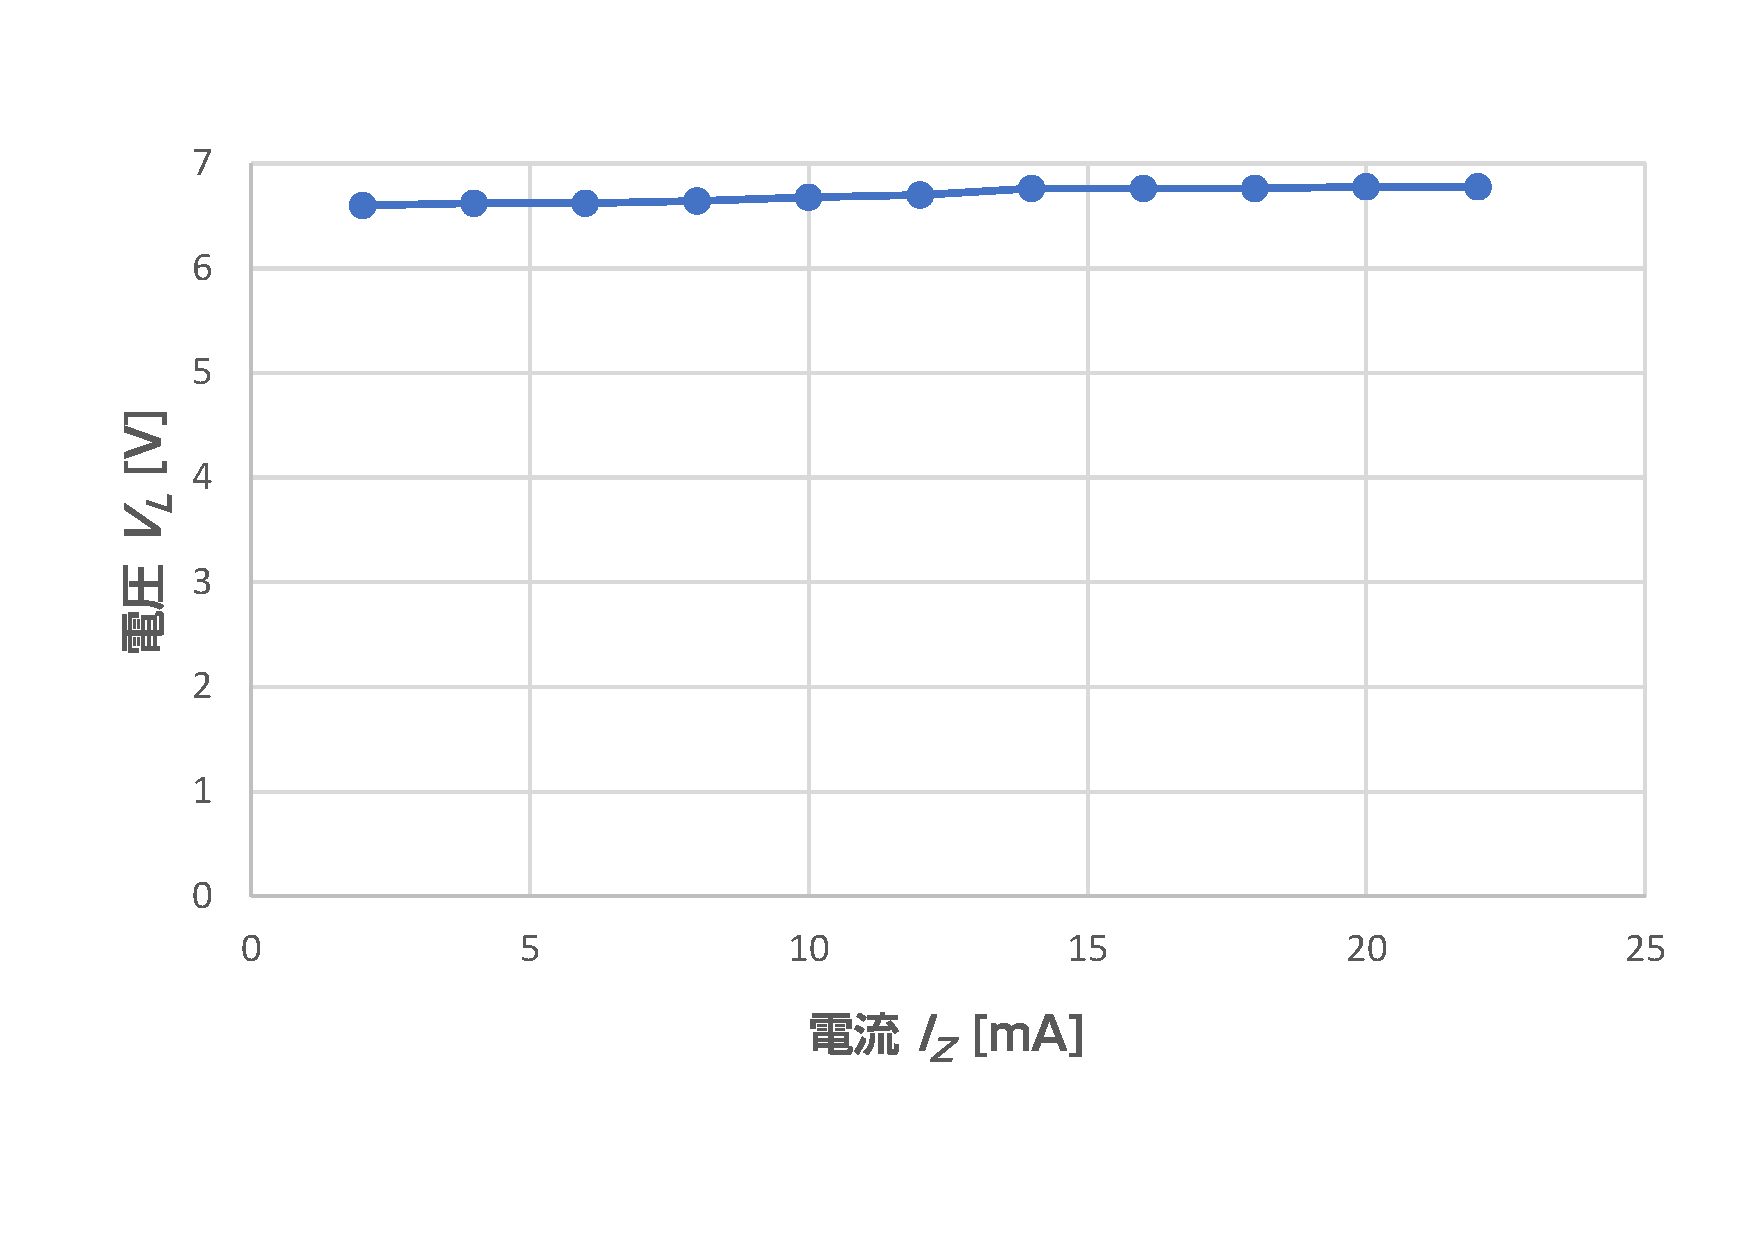
\includegraphics[width=13cm]{./figs/G-zener_IZ-VL.pdf}
		\caption{ツェナーダイオードの電流出力電圧特性}
		\label{fig:zener_IZ-VL}
	\end{figure}
	\begin{figure}[!h]
		\centering
		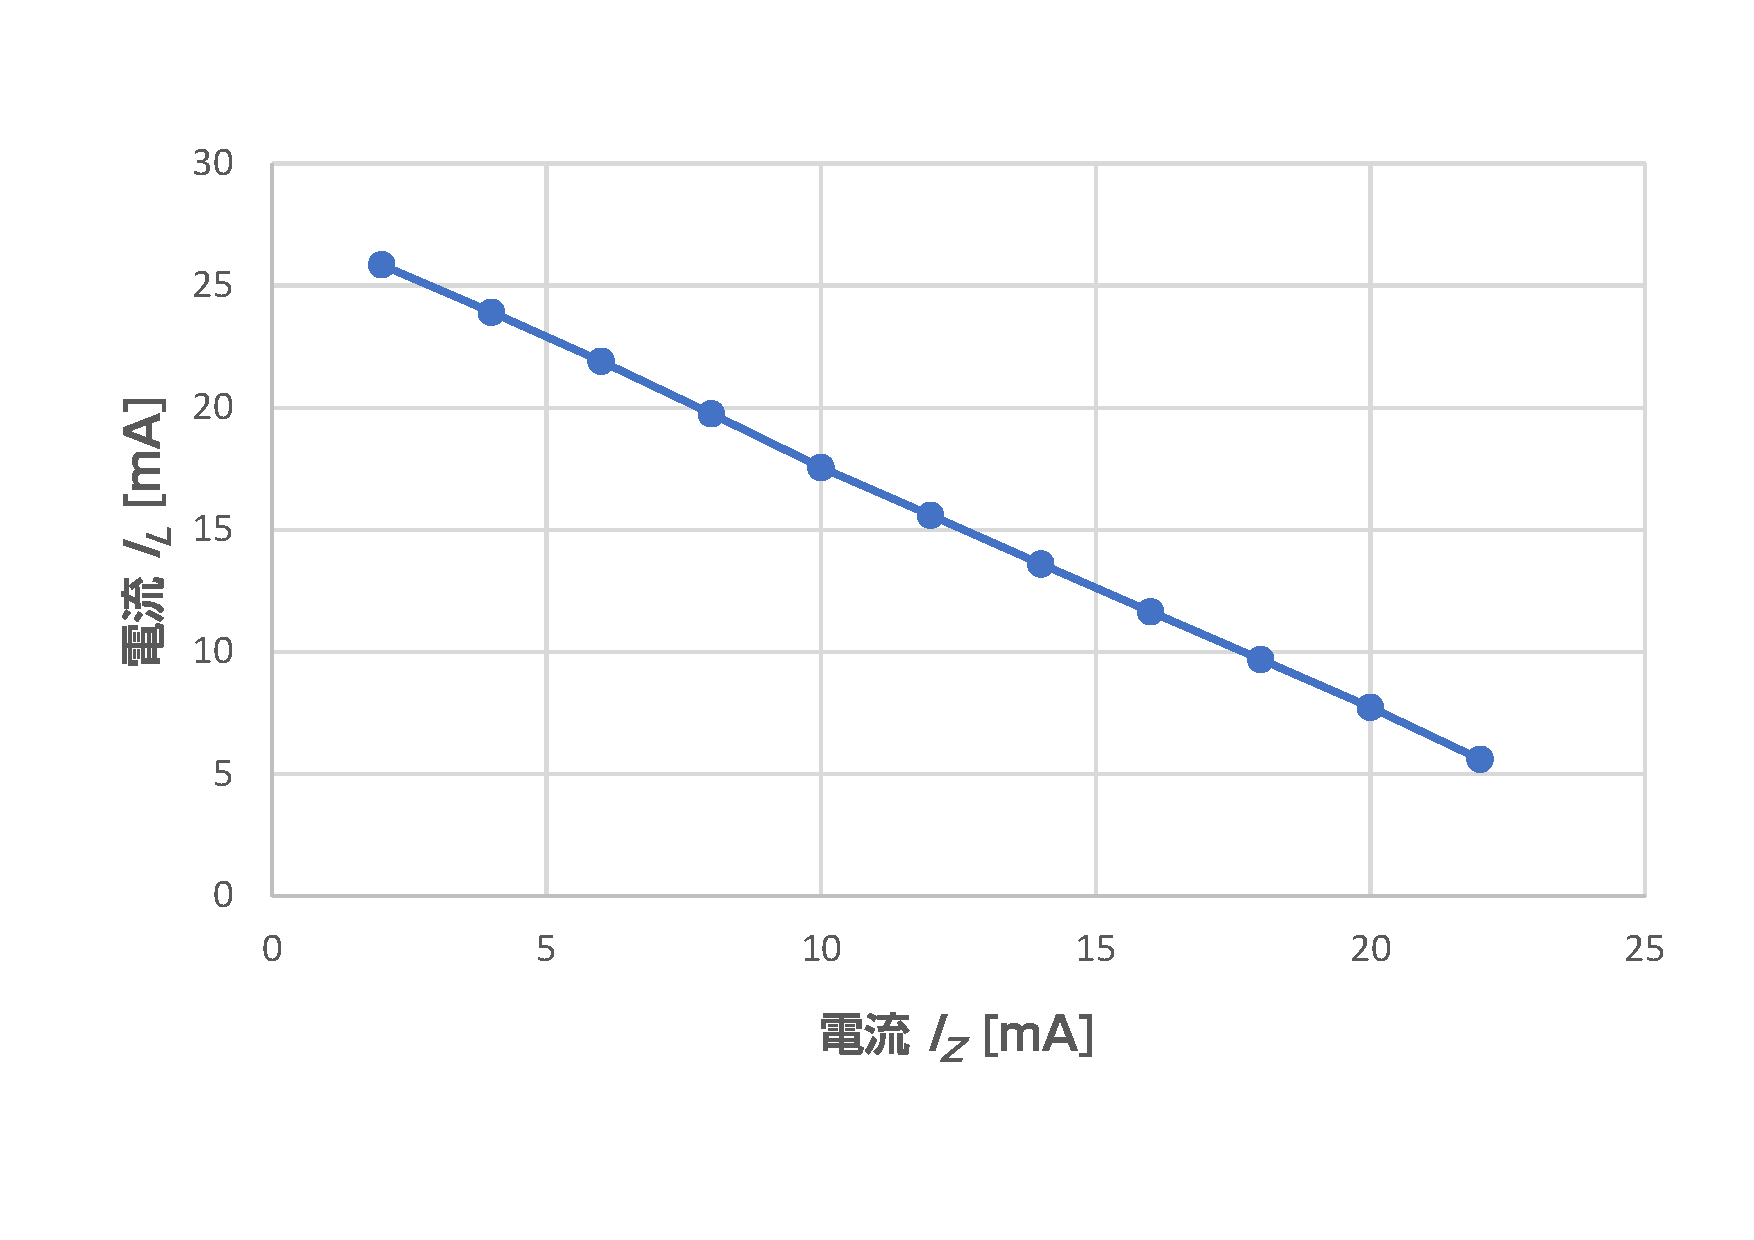
\includegraphics[width=13cm]{./figs/G-zener_IZ-IL.pdf}
		\caption{ツェナーダイオードの電流出力電流特性}
		\label{fig:zener_IZ-IL}
	\end{figure}

\subsubsection{考察}
	\begin{enumerate}
		\item 測定結果から,$R_L$,$R_Z$,およびこれらの合成抵抗 $R_A$ を算出せよ。\\
  
		\wfig{risou2} はツェナーダイオード定電圧回路の等価回路である。
		$ZD$は理想ツェナーダイオードであり,$R_Z$はツェナーダイオードの抵抗成分を示す。
		
				\begin{figure}[!h]
					\centering
					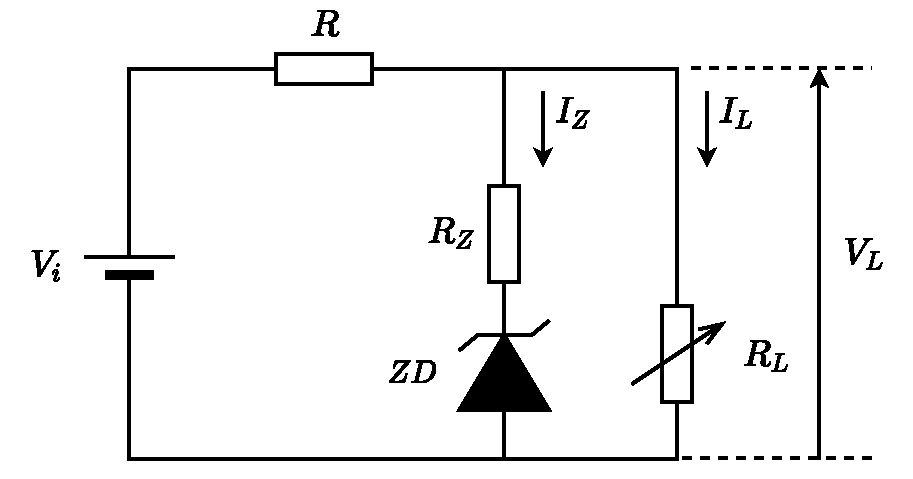
\includegraphics[width=8.2cm]{./pdfs/risou2.pdf}
					\caption{ツェナーダイオード定電圧回路の等価回路}
					\label{fig:risou2}
				\end{figure}
		
		$R_Z$,$R_L$は以下の式で求められる。
		\begin{align}
			R_Z &= \frac{V_L}{I_Z} \nonumber \\
			R_L &= \frac{V_L}{I_L} \nonumber
		\end{align}
		合成抵抗$R_A$は以下の式で求められる。
		\begin{equation}
			R_A = \frac{R_Z R_L}{R_Z + R_L} \nonumber
		\end{equation}
		これらの計算をそれぞれの計測点で行った結果を\wtab{resistance_calc1} に示す。
		\wtab{resistance_calc1} から合成抵抗$R_A$の抵抗値は,ほとんど変化していないと考えられる。

		\begin{table}[hbt]
			\centering
			\caption{$R_Z$,$R_L$,$R_A$の計算結果}
			\begin{tabular}{|c|c|c|c|}
			\hline
			電流$I_Z$ [mA] & 抵抗値$R_Z$ [k$\Omega$] & 抵抗値$R_L$ [k$\Omega$] & 合成抵抗$R_A$ [k$\Omega$] \\ \hline
			2               & 3.3              & 0.255319149      & 0.236984         \\ \hline
			4               & 1.655            & 0.276987448      & 0.237276         \\ \hline
			6               & 1.103333         & 0.302283105      & 0.237276         \\ \hline
			8               & 0.83             & 0.336202532      & 0.239279         \\ \hline
			10              & 0.668            & 0.380626781      & 0.242468         \\ \hline
			12              & 0.558333         & 0.429487179      & 0.242754         \\ \hline
			14              & 0.482857         & 0.497058824      & 0.244928         \\ \hline
			16              & 0.4225           & 0.580257511      & 0.244485         \\ \hline
			18              & 0.375556         & 0.696907216      & 0.244043         \\ \hline
			20              & 0.339            & 0.87483871       & 0.244324         \\ \hline
			22              & 0.308182         & 1.210714286      & 0.245652         \\ \hline
			\end{tabular}
			\label{tab:resistance_calc1}
		\end{table}

		\item $I_Z$ - $R_L$特性,$I_Z$ - $R_Z$特性を同一グラフに重ねて描き,考察せよ。\\
  
		\wtab{resistance_calc1} から作成したグラフを\wfig{zener_IZ-RZRL} に示す。
		\wfig{zener_IZ-RZRL} からツェナー電流$I_Z$が増加すると,$R_Z$は減少し,$R_L$は増加することが分かる。
		ツェナー電流$I_Z$が$\infty$まで増加させた時の,$R_Z$の値を考える。%また$R_L$の値も考える。

		$R_Z$は以下の式から考えられる。
		\begin{equation}
			R_Z = \frac{V_L}{I_Z} \nonumber
		\end{equation}
		この式の内,$V_L$は\wfig{zener_IZ-VL} の通り,ほぼ一定である。
		$I_Z$を$\infty$まで増加させたとすると,$R_Z$は0 [$\Omega$] になると考えられる。

		実際は,$I_Z$を$\infty$まで増加させてしまうと素子が燃えてしまうので,$R_Z$が0 [$\Omega$]になることはないと,考えられる。

		% $R_L$は以下の式から考えられる。
		% \begin{align}
		% 	R_A &= \frac{R_Z R_L}{R_Z + R_L} \nonumber \\
		% 	R_A(R_Z + R_L) &= R_Z R_L \nonumber \\
		% 	R_A R_L - R_Z R_L &= - R_A R_Z \nonumber \\
		% 	R_L &= \frac{R_A R_Z}{R_Z - R_A} \nonumber
		% \end{align}
		% この式に$R_Z = \frac{V_L}{I_Z}$を代入すると,

		\begin{figure}[!h]
			\centering
			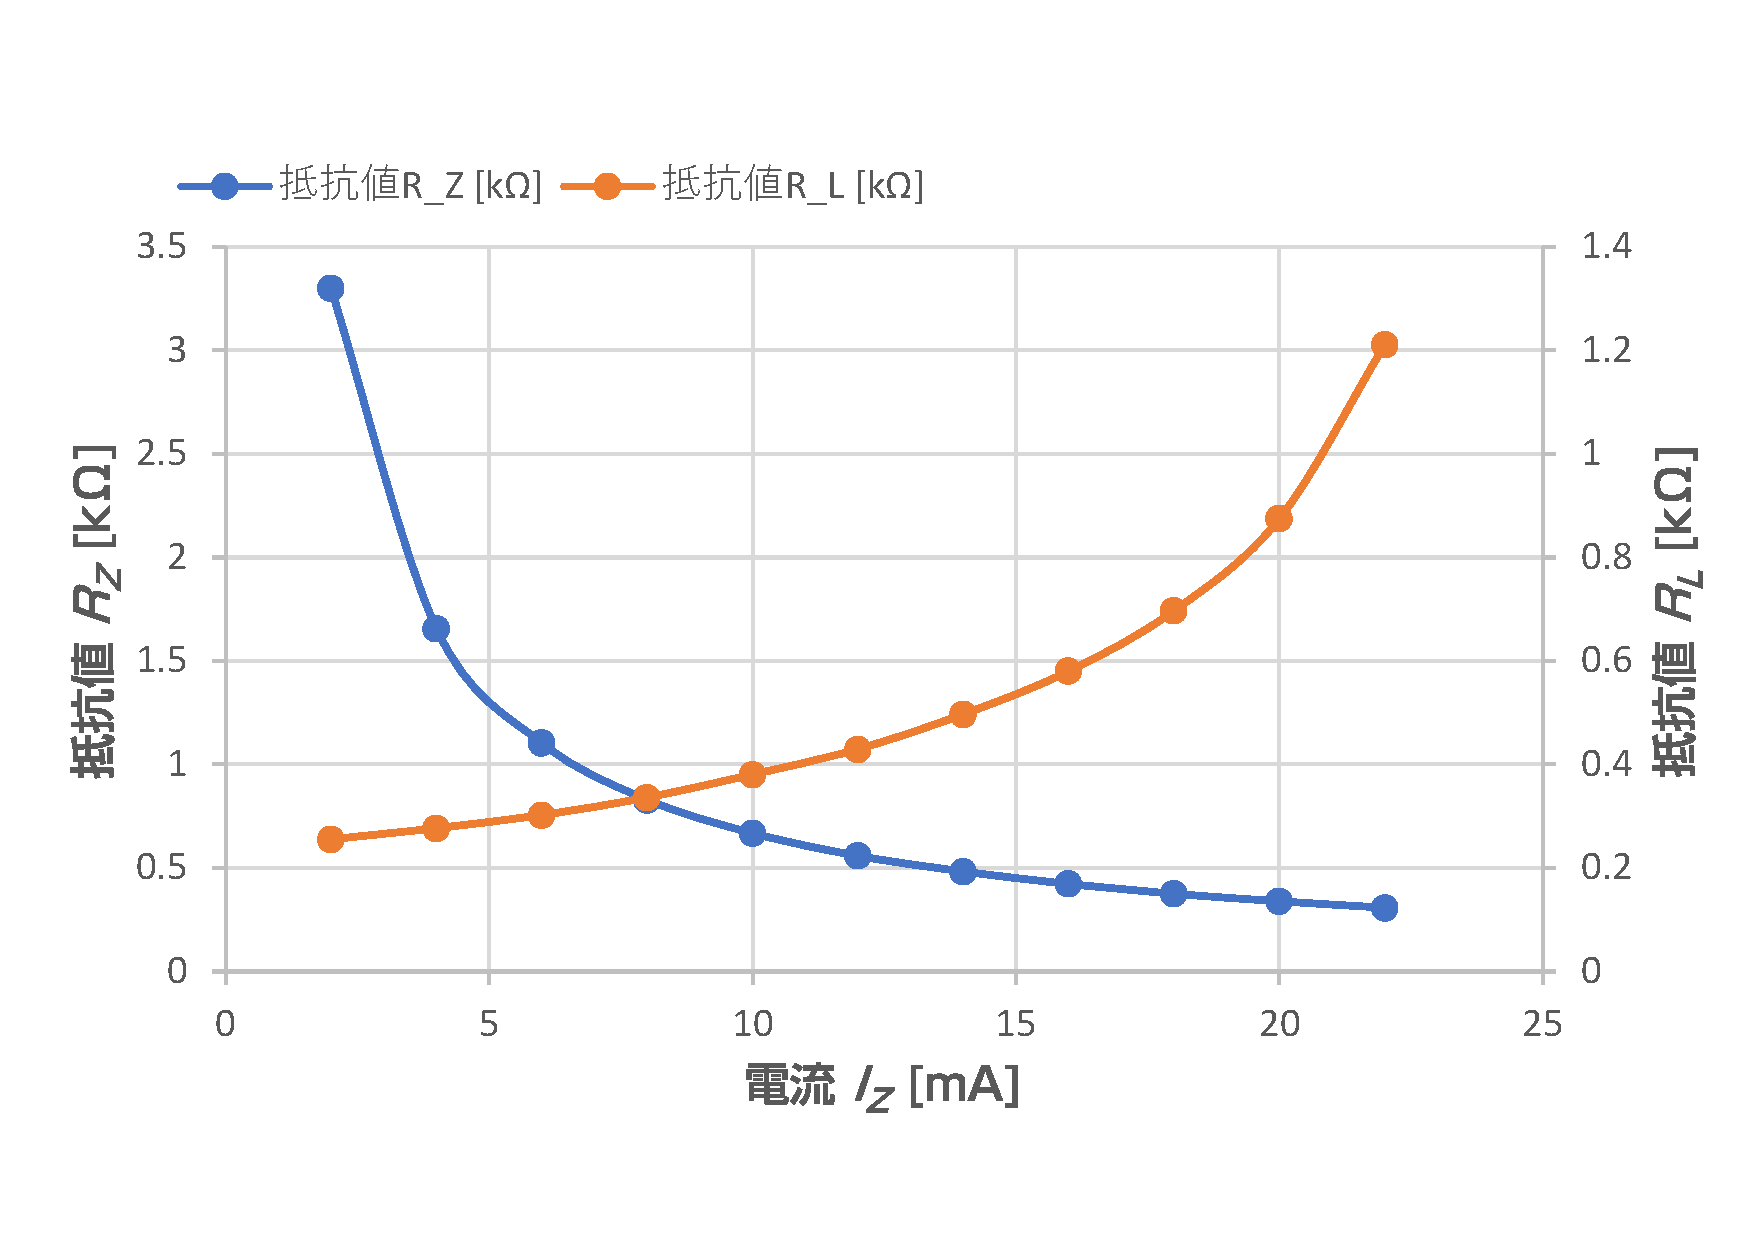
\includegraphics[width=13cm]{./figs/G-zener_IZ-RZRL.pdf}
			\caption{ツェナーダイオードの抵抗値電流特性}
			\label{fig:zener_IZ-RZRL}
		\end{figure}

	\end{enumerate}

\section{太陽電池の特性実験}
\subsection{使用器具}
太陽電池の特性実験の使用機材を以下のに示す
	\begin{table}[hbpt]
		\centering
		 表1:使用器具\\
			\begin{tabular}{|c||c|c|c|} \hline
			使用器具名 & 製造元 & 型番 & 製造番号(管理番号)\\ \hline
			 & 5 & 3 & \\ \hline
			 & 1 & 8 & \\ \hline
			 & 1 & 8 & \\ \hline
			\end{tabular}

	\end{table}

\subsection{太陽電池の発電特性}
\subsubsection{実験方法}
\subsubsection{結果}
\subsubsection{考察}


\subsection{実験手順}


\section{結果}
\section{考察}
\section{結論}

\begin{thebibliography}{9}%参考文献数が10以上の場合は9を99に変更
	\bibitem{tyosho:denkiKiso1} 堀田栄喜,電気基礎1 新訂版,実教出版株式会社,東京,2020
	\bibitem{tyosho:densiKairo} 高木茂孝,電子回路 新訂版,実教出版株式会社,東京,2022
	\bibitem{web:1N4001} ``1N4001, 1N4002, 1N4003, 1N4004, 1N4005, 1N4006, 1N4007'',vishay,\url{https://www.vishay.com/docs/88503/1n4001.pdf},2022/05/18
	\bibitem{web:1N4736A} ``Zener Diodes 1N4728A - 1N4758A'',onsemi,\url{https://www.onsemi.com/pdf/datasheet/1n4736at-d.pdf},2022/05/18
	\bibitem{web:reverse_current} ``39.ダイオードの基本'',chip one stop,\url{https://www.chip1stop.com/sp/knowledge/039_fundamentals-of-diodes#:~:text=%E5%AE%9F%E9%9A%9B%E3%81%AE%E3%83%80%E3%82%A4%E3%82%AA%E3%83%BC%E3%83%89%E3%81%A7%E3%81%AF%E3%80%81%E9%80%86,%E6%B5%81%E3%82%8C%E3%82%8B%E3%82%88%E3%81%86%E3%81%AB%E3%81%AA%E3%82%8A%E3%81%BE%E3%81%99%E3%80%82},2022/05/18
\end{thebibliography}% 参考文献


\end{document}

